\section{Detector Performance}

In order to calibrate the detectors and test their performance, a cosmic-ray test bench was designed and installed at Saclay
early in the project. The goal of these tests was to determine the best operating conditions
of the detectors and to compute their 2D efficiency maps using cosmic muons prior shipment to JLab.

\begin{figure}[htb]
 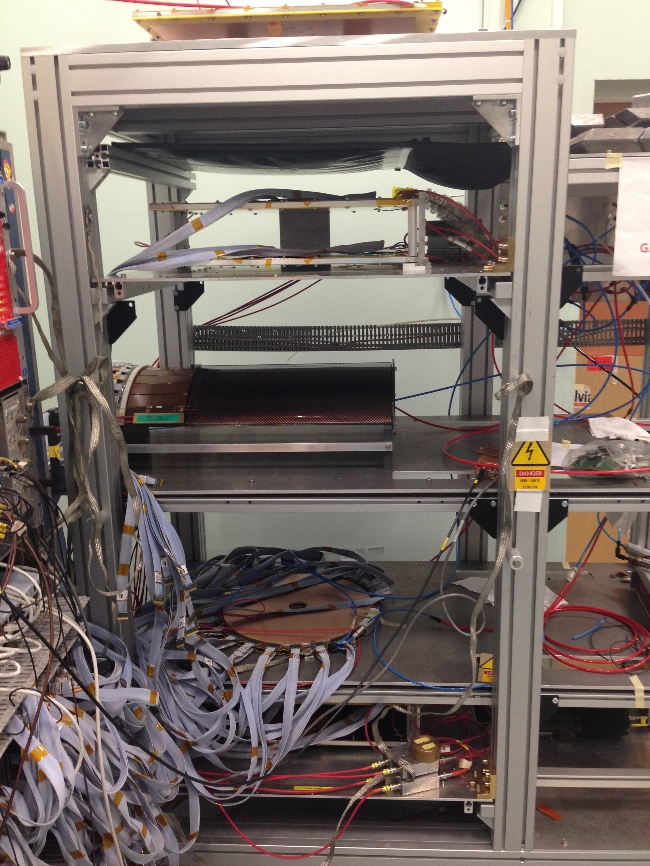
\includegraphics[width=1.0\columnwidth,keepaspectratio]{images/banc_cosmique}
 \caption{The cosmic bench made of an external trigger from the coincidence of two scintillators and a hodoscope made of 4 
reference trackers. The photograph shows the simultaneous operation of a BMT tile and a FMT disk under test.}
 \label{fig:mm-testbench}
\end{figure}

The cosmic-ray test bench shown in Fig.~\ref{fig:mm-testbench} consists of a vertical stack of six detectors. Two scintillators
are installed at the top and the bottom of the stack to provide the trigger. Four $50 \times 50 \text{ cm}^2$ double-layer flat
Micromegas were used as a tracker to provide the reference track of a cosmic ray. In the middle of the stack, empty trays
receive the detectors to be characterized.

After alignment of the reference trackers and the detectors to be tested, the expected position of the particle in the test
detector was provided by the reference trackers and compared with the measured signals, if any, in the test detector. If a
signal matched the expected position within a millimeter, the test detector was considered to have seen the cosmic ray. The
efficiency was then derived by repeating this test over a cosmic ray sample collected within a few hours. All MVT detectors
were systematically characterized before shipment to JLab. These tests included a study of the efficiency as a function of
the amplification voltage and a two-dimensional efficiency map, which required a cosmic ray sample collected over a day.

The results were found to be similar for all detectors. The efficiency plateau starts at about 500~V with a value between
98.5\% and 99.5\% at 510~V. It was shown that the plateau was slightly shifted to higher strip voltages when the drift plane
was at higher voltage because the mesh loses electron transparency. The 2D-efficiency map was useful to look for any structural
problems. All MVT detectors that were shipped to JLab had a uniform 2D-efficiency map. Examples of the efficiency plateau
and the 2D efficiency map are shown in Figs.~\ref{fig:mm-fig8} and \ref{fig:mm-fig9}. Figure \ref{fig:mm-fig9} shows the
efficiency gain by removing the protection diodes in front of the front-end Dream ASICs. Since the resistive Micromegas
technology was used, sparks are quenched and protection of the front-end electronics is no longer required (beside the chip
packaging protection) even with high gain in beam conditions.

\begin{figure}[htb]
 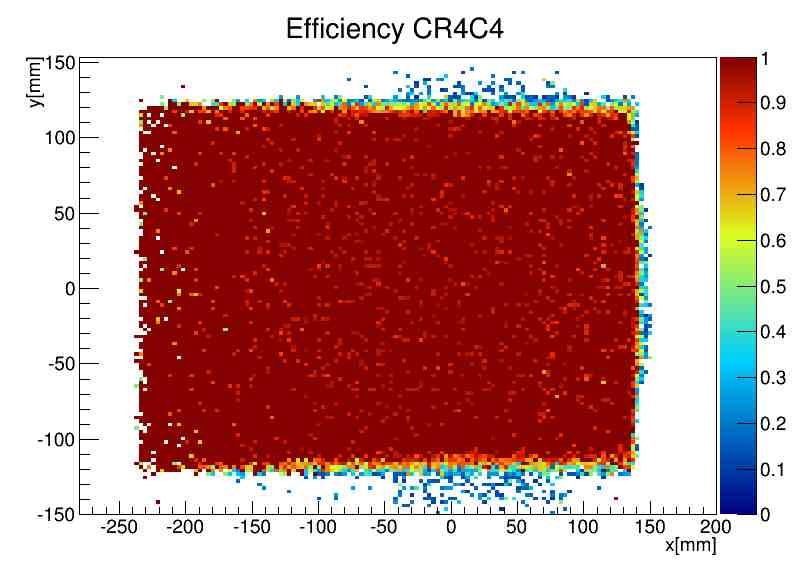
\includegraphics[width=1.0\columnwidth,keepaspectratio]{images/Eff_2D}
 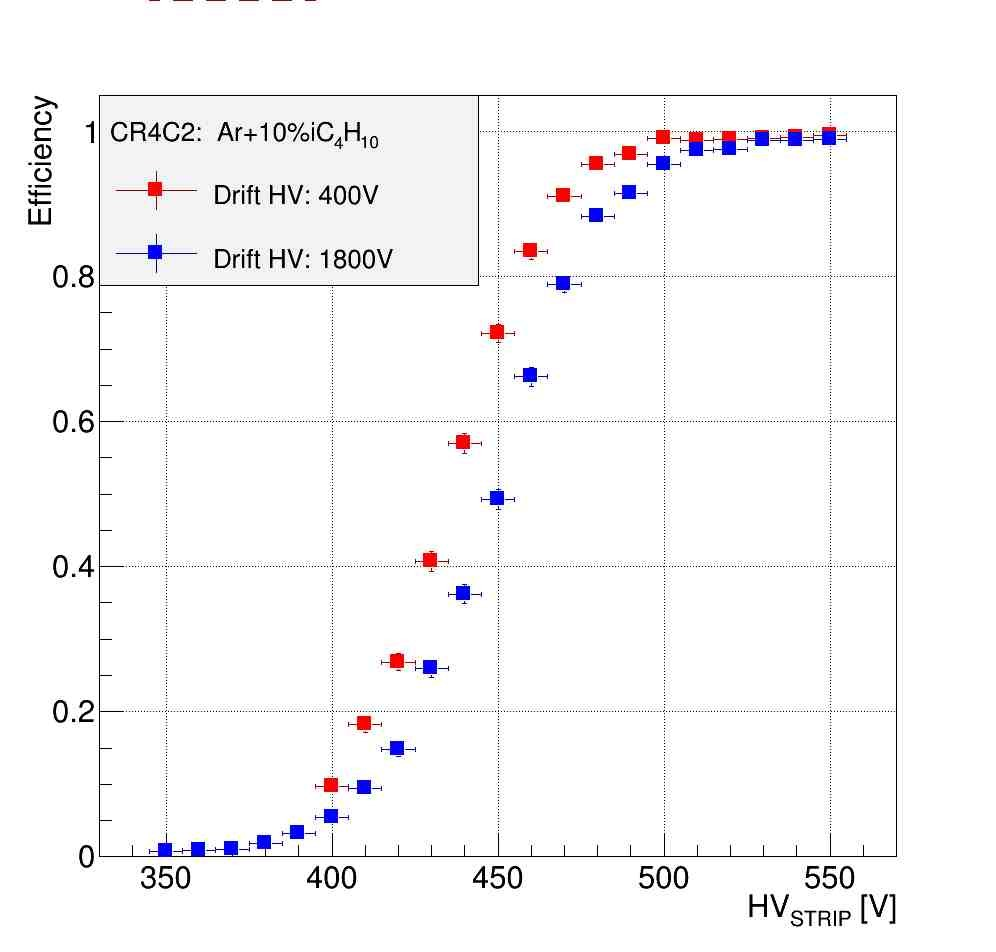
\includegraphics[width=1.0\columnwidth,keepaspectratio]{images/Plateau_HV}
 \caption{Efficiency plateau (bottom) and 2D efficiency map (top) for a C-type barrel detector.}
 \label{fig:mm-fig8}
\end{figure}

\begin{figure}[htb]
 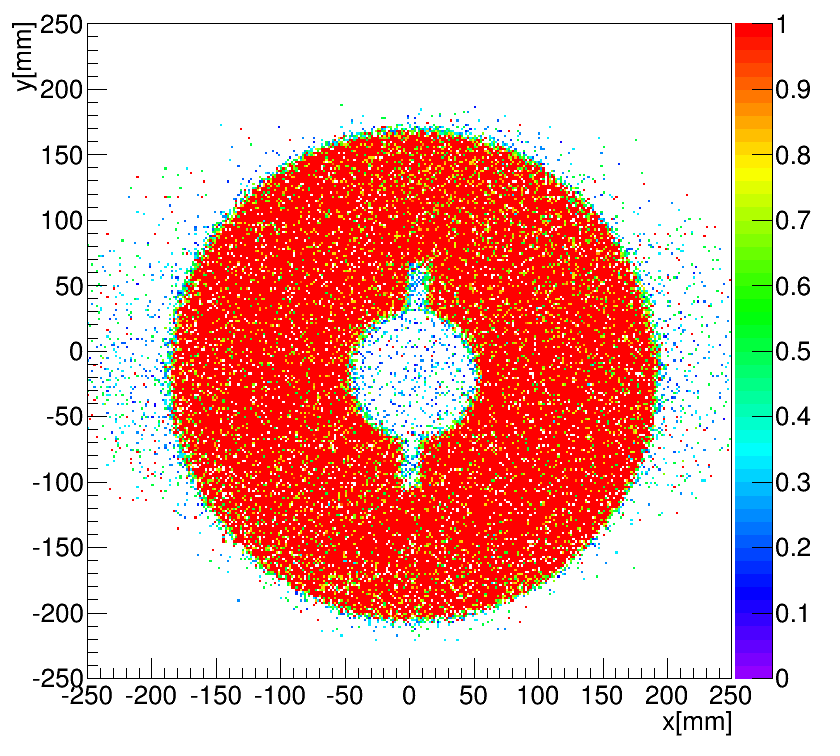
\includegraphics[width=1.0\columnwidth,keepaspectratio]{images/FMT_eff_2Dmap_testBench.png}
 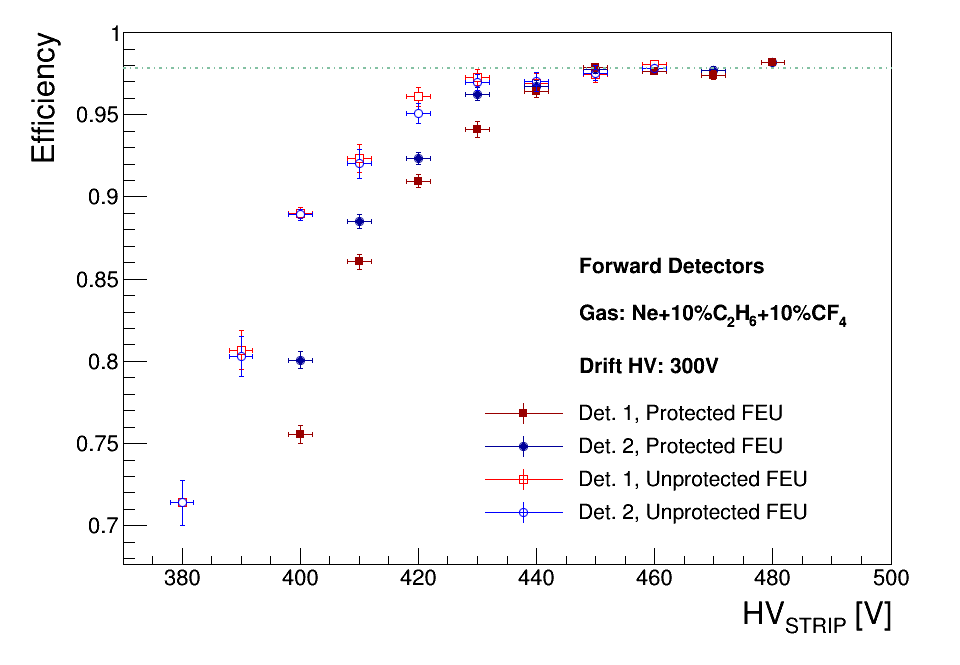
\includegraphics[width=1.0\columnwidth,keepaspectratio]{images/FMT_eff_plateau_testBench.png}
 \caption{Efficiency plateau (bottom) and 2D efficiency map (top) for a FMT disk.}
 \label{fig:mm-fig9}
\end{figure}

\subsection{Commissioning}

The Micromegas Vertex Tracker was delivered to JLab in June 2017. A team of 10 people assembled the MVT and integrated
it with the SVT to form the final configuration of the CLAS12 Central Vertex Tracker. The MVT barrel was first commissioned
with cosmic rays in the assembly room until mid-October 2017 and for the first two weeks after it was installed in Hall~B. The
final phase of the commissioning started in December 2017 with beam.

Before the start of data taking with beam, several cosmic ray runs were performed aimed at tuning and optimizing the
integration of the data acquisition system and the slow-controls (i.e. remote controls, interlocks, and 
monitoring)~\cite{daq-nim},
and the gas delivery system. The online data monitoring system was developed to allow the inspection of raw quantities such as the
hit maps, the pulse shape, and the timing of the signals. This system was tested and integrated into the standard CLAS12
online operation tools. 

\subsection{Cosmic Ray Data Taking}
\label{sec:cosmics}

Cosmic-ray data with zero magnetic field were used not only for commissioning purposes, but also for the essential detector
alignment. Given the absence of the solenoid magnetic field, the drift high voltages were set to about 400~V as the primary
electrons do not experience the Lorentz-angle effect. The cosmic ray trigger for the Central Detector was provided by
coincidences of CTOF signals in diametrically opposed scintillator bars. This CTOF trigger provides a quasi-uniform
illumination along the BMT axis of the barrel with cosmic rays, not achievable in beam conditions because of the forward-peaked
distribution due to the center-of-mass boost. The hit distribution on the Z-tiles, instead, results from a convolution of the cosmic
ray angular distribution with the trigger configuration. As is shown in Fig.~\ref{fig:mm-cosmic_occupancy}, sector~2 has about
twice as many hits as sector~1 and 3 since it is centered at the top of the barrel.

\begin{figure}[htb]
 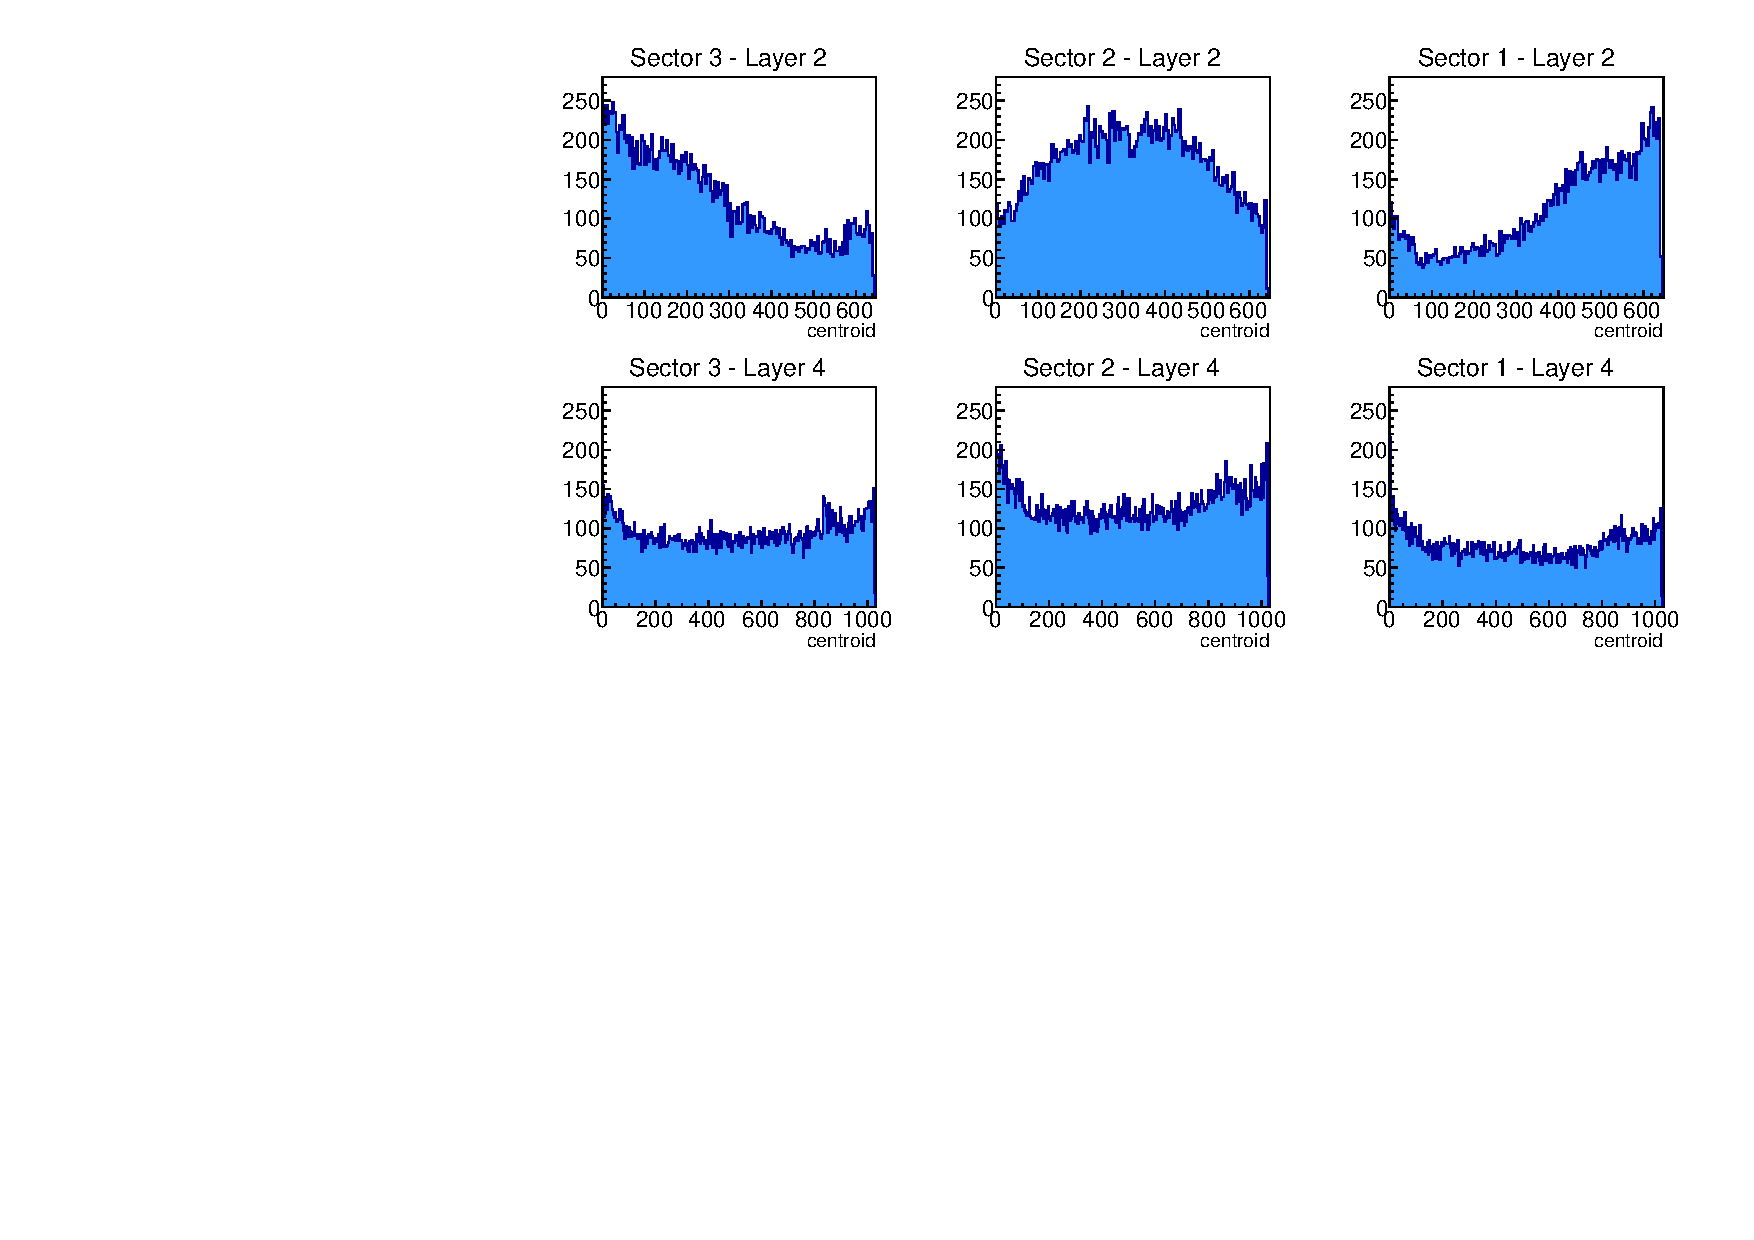
\includegraphics[width=.45\textwidth]{images/BMT_hit_cosmics_CTOFtrigger.pdf}
 \caption{Hit occupancies of a cosmic-ray run with the trigger delivered by the CTOF for layers 3 (Z-tile) and 4 (C-tile).}
 \label{fig:mm-cosmic_occupancy}
\end{figure}

The distributions of cluster size for the three sectors (see Fig.~\ref{fig:mm-cosmic_cls}) show, on average, larger clusters in
sector~1 and 3 with respect to sector~2. Indeed, since cosmic rays are mostly vertical, the projection of their path in the drift
gap onto the strip surface is longer for sectors~1 and 3 than for sector~2.

\begin{figure}[htb]
 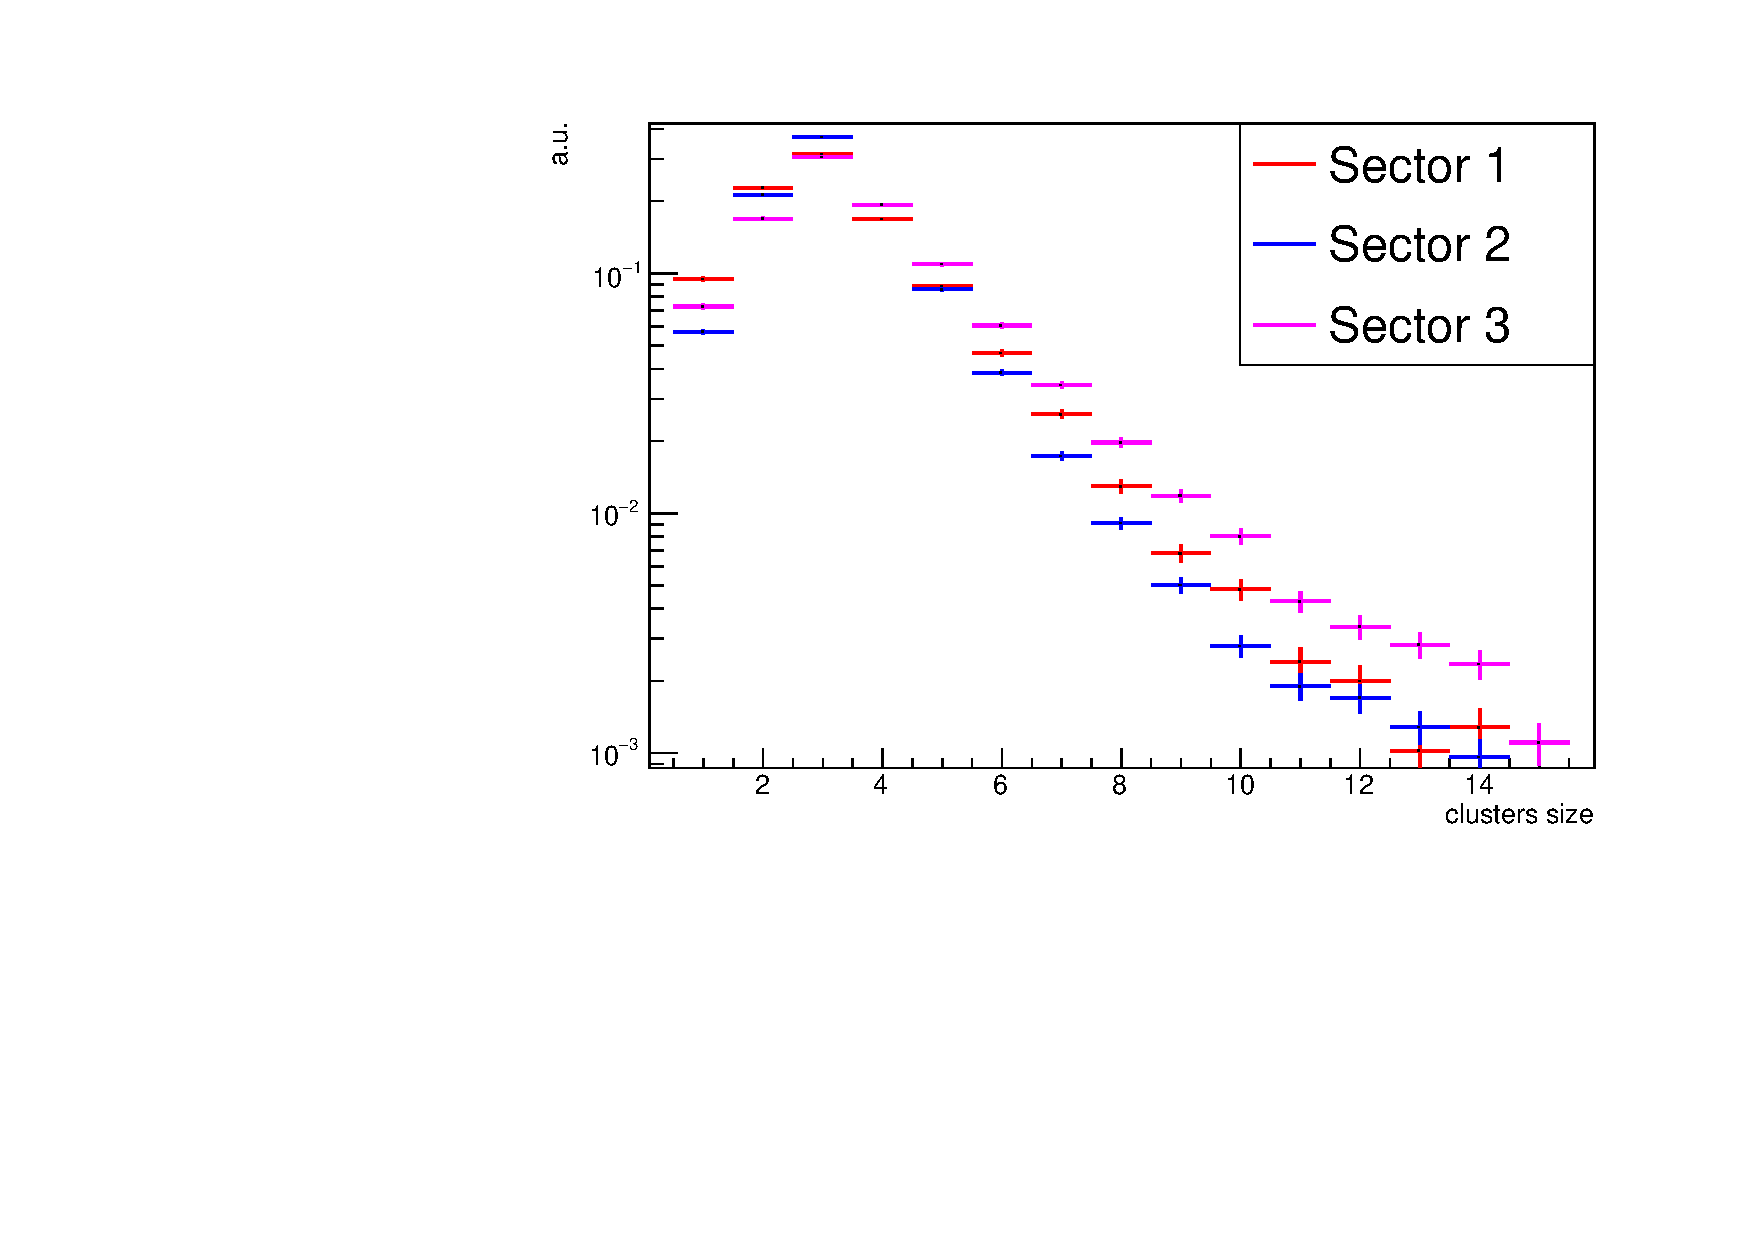
\includegraphics[width=.45\textwidth]{images/cosmic_cluster_size.pdf}
 \caption{Cluster size distributions during cosmic ray data taking for the three sectors.}
 \label{fig:mm-cosmic_cls}
\end{figure}

A BMT stand-alone straight-track reconstruction algorithm based on least-squares minimization has been developed to reconstruct
cosmic rays. A typical reconstructed event is shown in Fig.~\ref{fig:mm-cosmic_ced} using the CLAS12 event display package
\cite{recon-nim}. This tracking algorithm is also used to perform the alignment of the BMT tiles: the distance between 
the hit in a
tile excluded from the tracking and the reference track provided by the other tiles is minimized by introducing rotations and
translations. Figure~\ref{fig:mm-cosmic_residuals} shows the distributions of track residuals, i.e. the distance of a hit with
respect to the particle trajectory, for three Micromegas tiles before and after alignment corrections.
Figure~\ref{fig:mm-cosmic_res_summary} shows the summary of the preliminary results for all BMT detectors: after the
alignment procedure all residual distributions are centered around zero. Preliminary detector resolutions, defined as the standard
deviations of Gaussian fits to the residual distributions, are improved and below 200~$\mu$m. 

\begin{figure}[htb]
 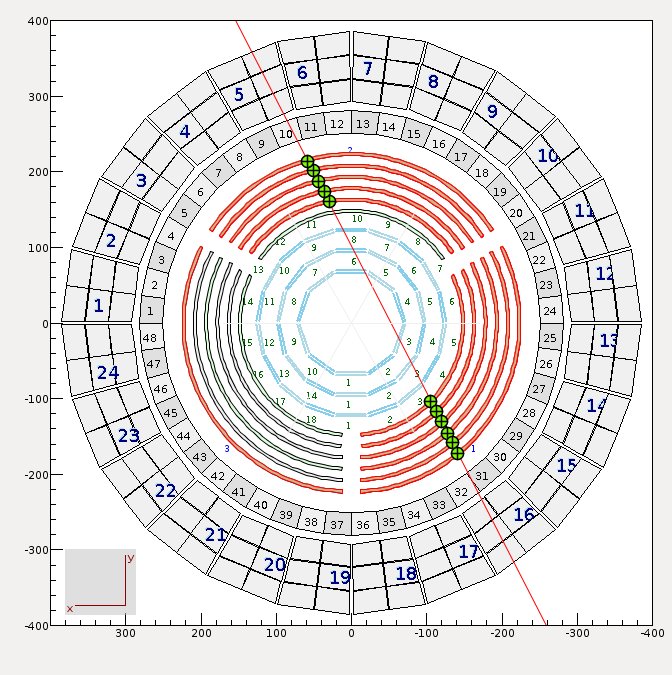
\includegraphics[width=.4\textwidth]{images/cosmic_NIM.png}
 \caption{Event display of a cosmic ray track reconstructed in the BMT detectors.}
 \label{fig:mm-cosmic_ced}
\end{figure}

\begin{figure}[htb]
 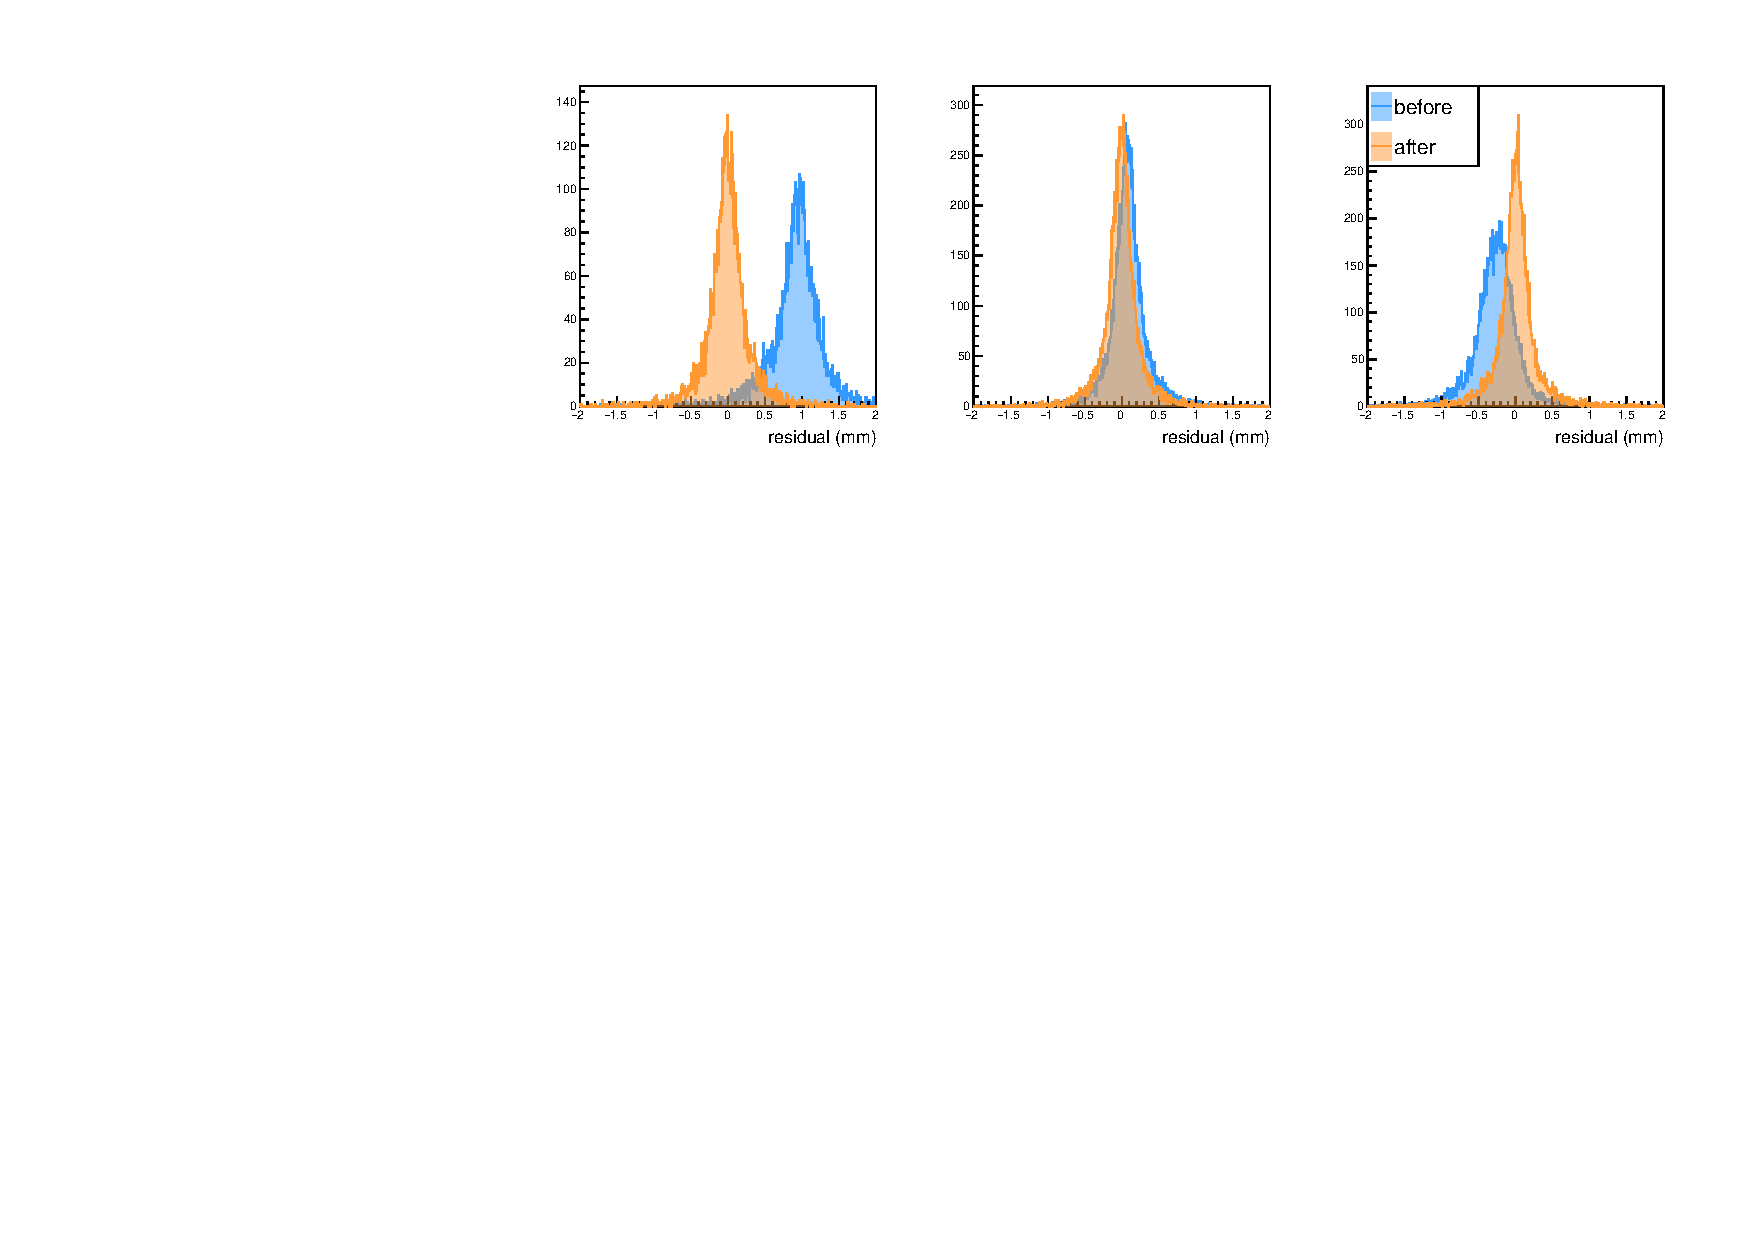
\includegraphics[width=.45\textwidth]{images/cosmic_residuals.pdf}
 \caption{Example of residuals for three BMT tiles with cosmic ray data before and after a preliminary alignment procedure
   obtained with a BMT stand-alone reconstruction.}
 \label{fig:mm-cosmic_residuals}
\end{figure}

\begin{figure}[htb]
 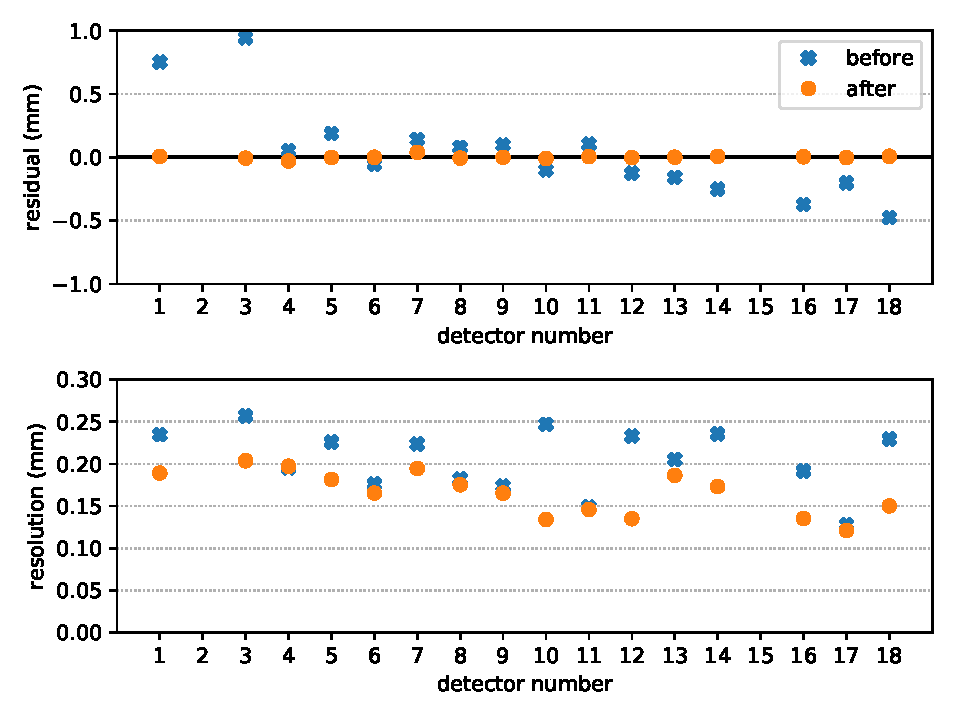
\includegraphics[width=\columnwidth]{images/residuals_and_resolutions.pdf}
 \caption{Preliminary BMT residuals (top) and resolutions (bottom) with cosmic-ray data before and after an alignment procedure
   obtained with a BMT stand-alone reconstruction.}
 \label{fig:mm-cosmic_res_summary}
\end{figure}

\subsection{Data Taking with Beam}

With the start of beam operations, the behavior of the detectors has been carefully monitored and the working parameters
such as high voltage settings have been tuned. The working point for the strip high voltage has been studied by performing a
scan with a 20~V step. Due to delays in the offline data reconstruction for a proper efficiency measurement, the cluster
multiplicity per electron trigger was used as an alternative observable accessible online that can be used to exhibit a plateau. 
Indeed, as shown in Fig.~\ref{fig:mm-fig15}, this observable was found to flatten out where the efficiency plateau was
determined from the commissioning with cosmic rays. For the FMT, the plateau was found from 460~V to 490~V. Above 490~V, the
cluster multiplicity and the current on the strips increases suddenly, potentially due to a Corona effect. It was decided to set
460~V as the nominal HV settings for the FMT, which allows safe operations at nominal luminosity. The nominal HV setting was
decided to be 520~V for the BMT, although the plateau was not as clear as for the FMT.  

%\begin{figure}[htb]
% 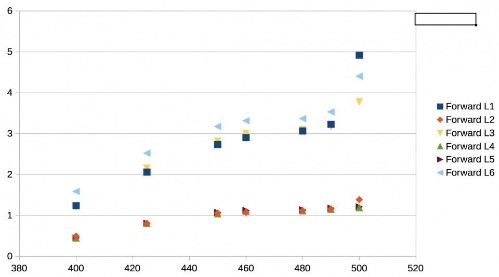
\includegraphics[width=1.0\columnwidth,keepaspectratio]{images/Plateau_cluster_FMT.jpg}
% \caption{Cluster multiplicity in FMT as a function of HV on the strips.}
% \label{fig:mm-fig15}
%\end{figure}
\begin{figure}[htb]
 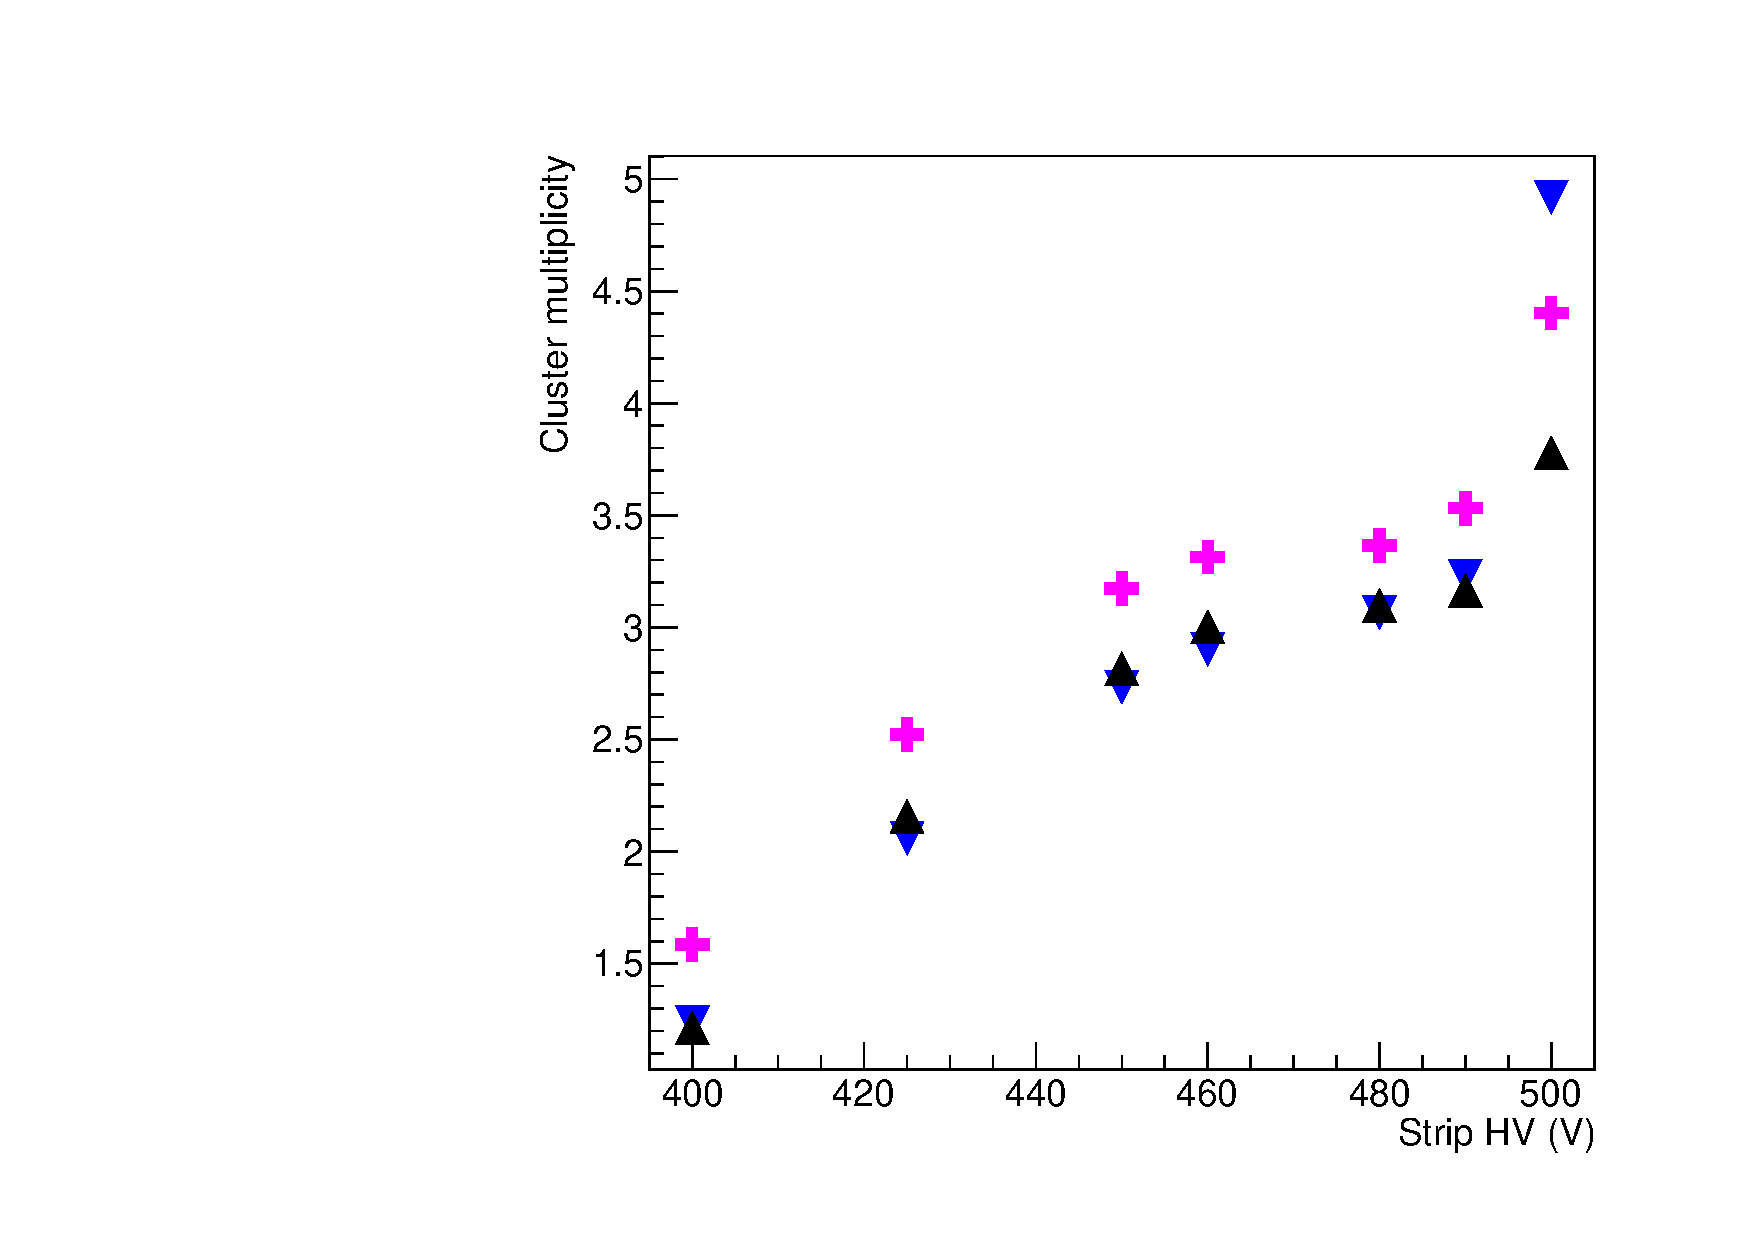
\includegraphics[width=1.0\columnwidth,keepaspectratio]{images/PseudoEfficiencies_ClusterMultiplicities_FMT_only3layers.pdf}
 \caption{Cluster multiplicity in 3 FMT disks as a function of HV on the strips.}
 \label{fig:mm-fig15}
\end{figure}

Preliminary efficiencies for the Micromegas detectors were measured by performing tracking without the detector under study
to determine for each track going through the studied detector, if a hit was found close to the expected intersection. The
efficiency plateau was found to be at the same position as the plateau with the cluster multiplicities, thus validating the HV
settings used. An example of the efficiency scan for one BMT tile is shown in Fig.~\ref{fig:mm-eff_scan}.

\begin{figure}[htb]
 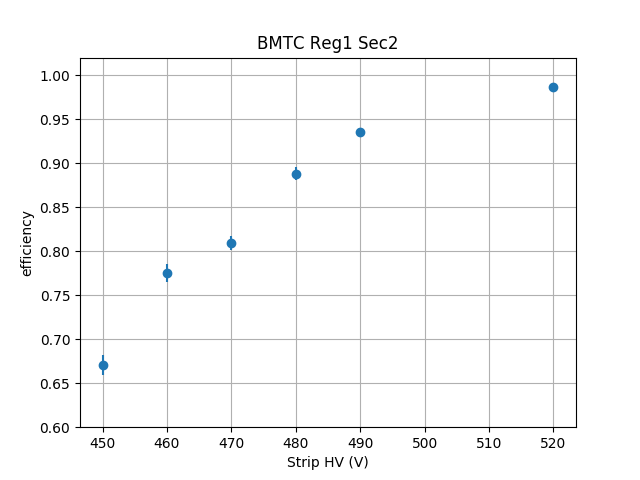
\includegraphics[width=1.0\columnwidth,keepaspectratio]{images/hvscan_BMTC_R1_S2.png}
 \caption{Efficiency measurement as a function of the strip high voltage for one tile in beam conditions.}
 \label{fig:mm-eff_scan}
\end{figure}

Strip currents and detector occupancy have been measured during a beam intensity scan up to the instantaneous luminosity of
about $10^{35}$~cm$^{-2}$s$^{-1}$. Figure~\ref{fig:mm-fig14} shows the correlation between the currents drawn by the BMT
strips and the beam current. The slope coefficient resulting from a linear regression is 0.02~$\mu$A/nA. At the maximum
beam current of 78~nA, two BMT tiles reached the safety threshold of 2~$\mu$A and they were automatically turned off. The
detector occupancy shows as well a linear correlation with the beam current, reaching values of about 3.5\% for the FMT disks
and 2.5\% for the BMT tiles at nominal luminosity, as shown in Fig.~\ref{fig:mm-fig16}.

\begin{figure}[htb]
 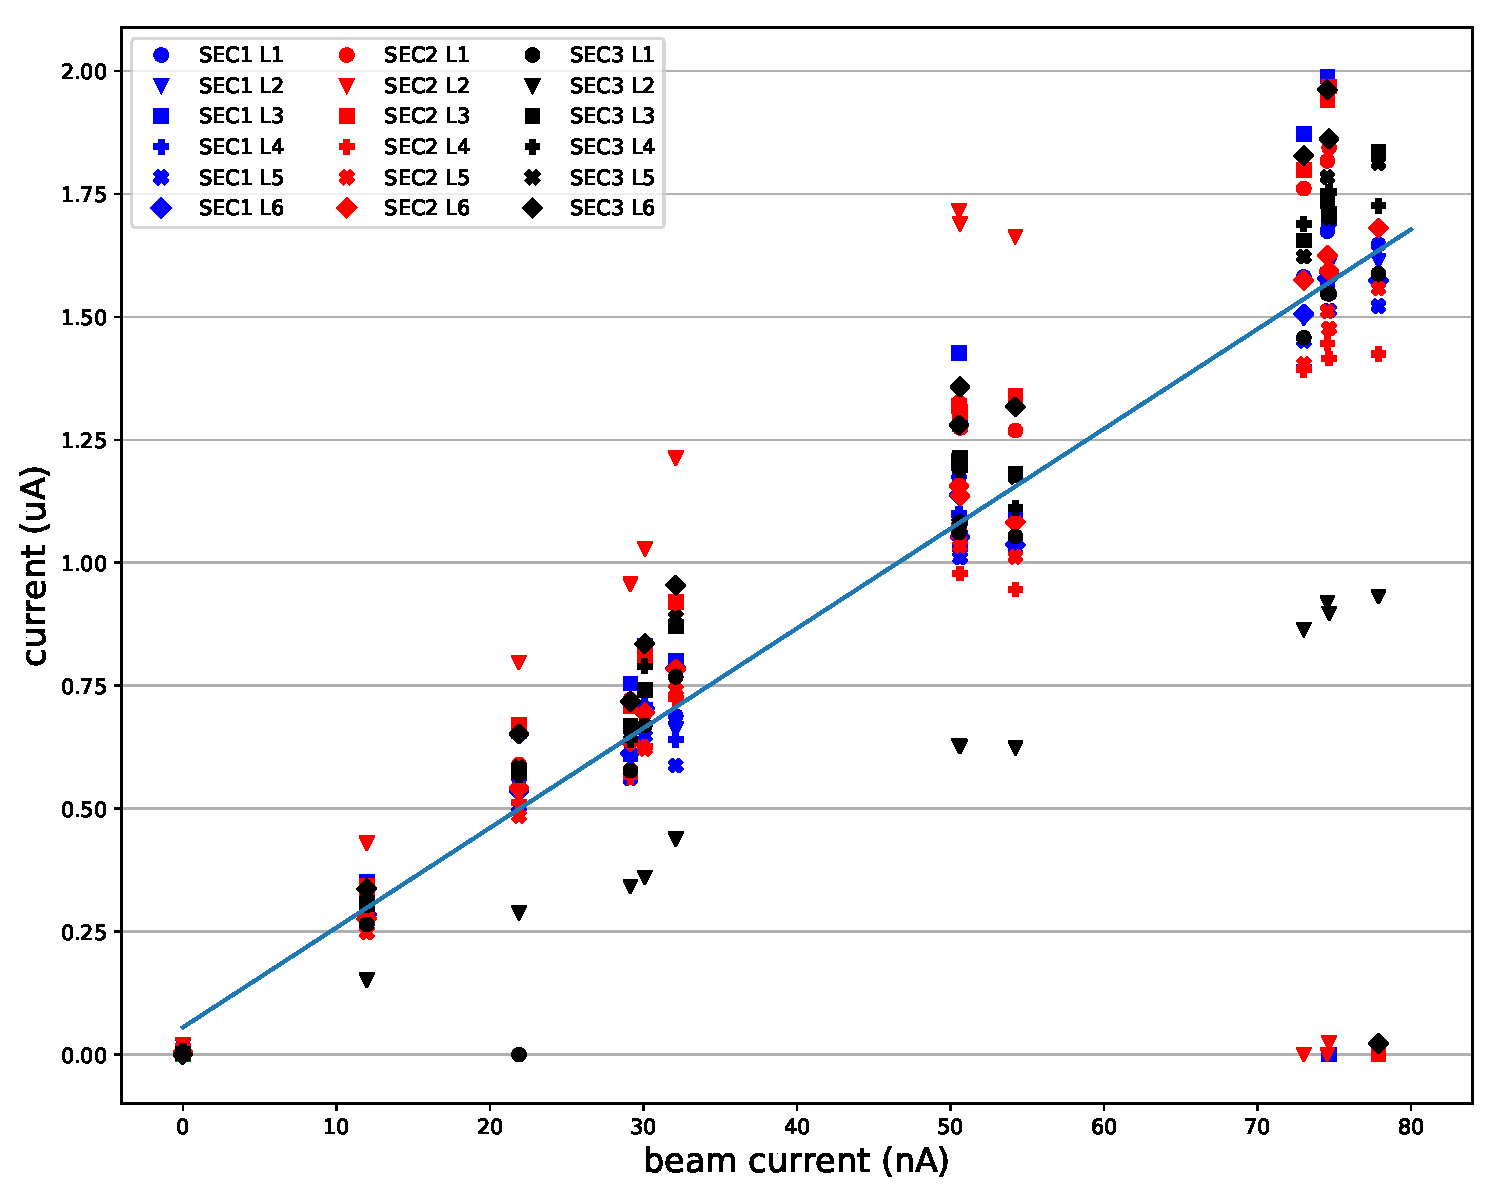
\includegraphics[width=1.0\columnwidth,keepaspectratio]{images/BMT_IvsLumi}
 \caption{Currents on the BMT strips as a function of beam current on a 5-cm-long liquid-hydrogen target. All detectors have similar
   currents. The nominal luminosity of $10^{35}$~cm$^{-2}$s$^{-1}$ corresponds to 75~nA on target.}
 \label{fig:mm-fig14}
\end{figure}

\begin{figure}[htb]
 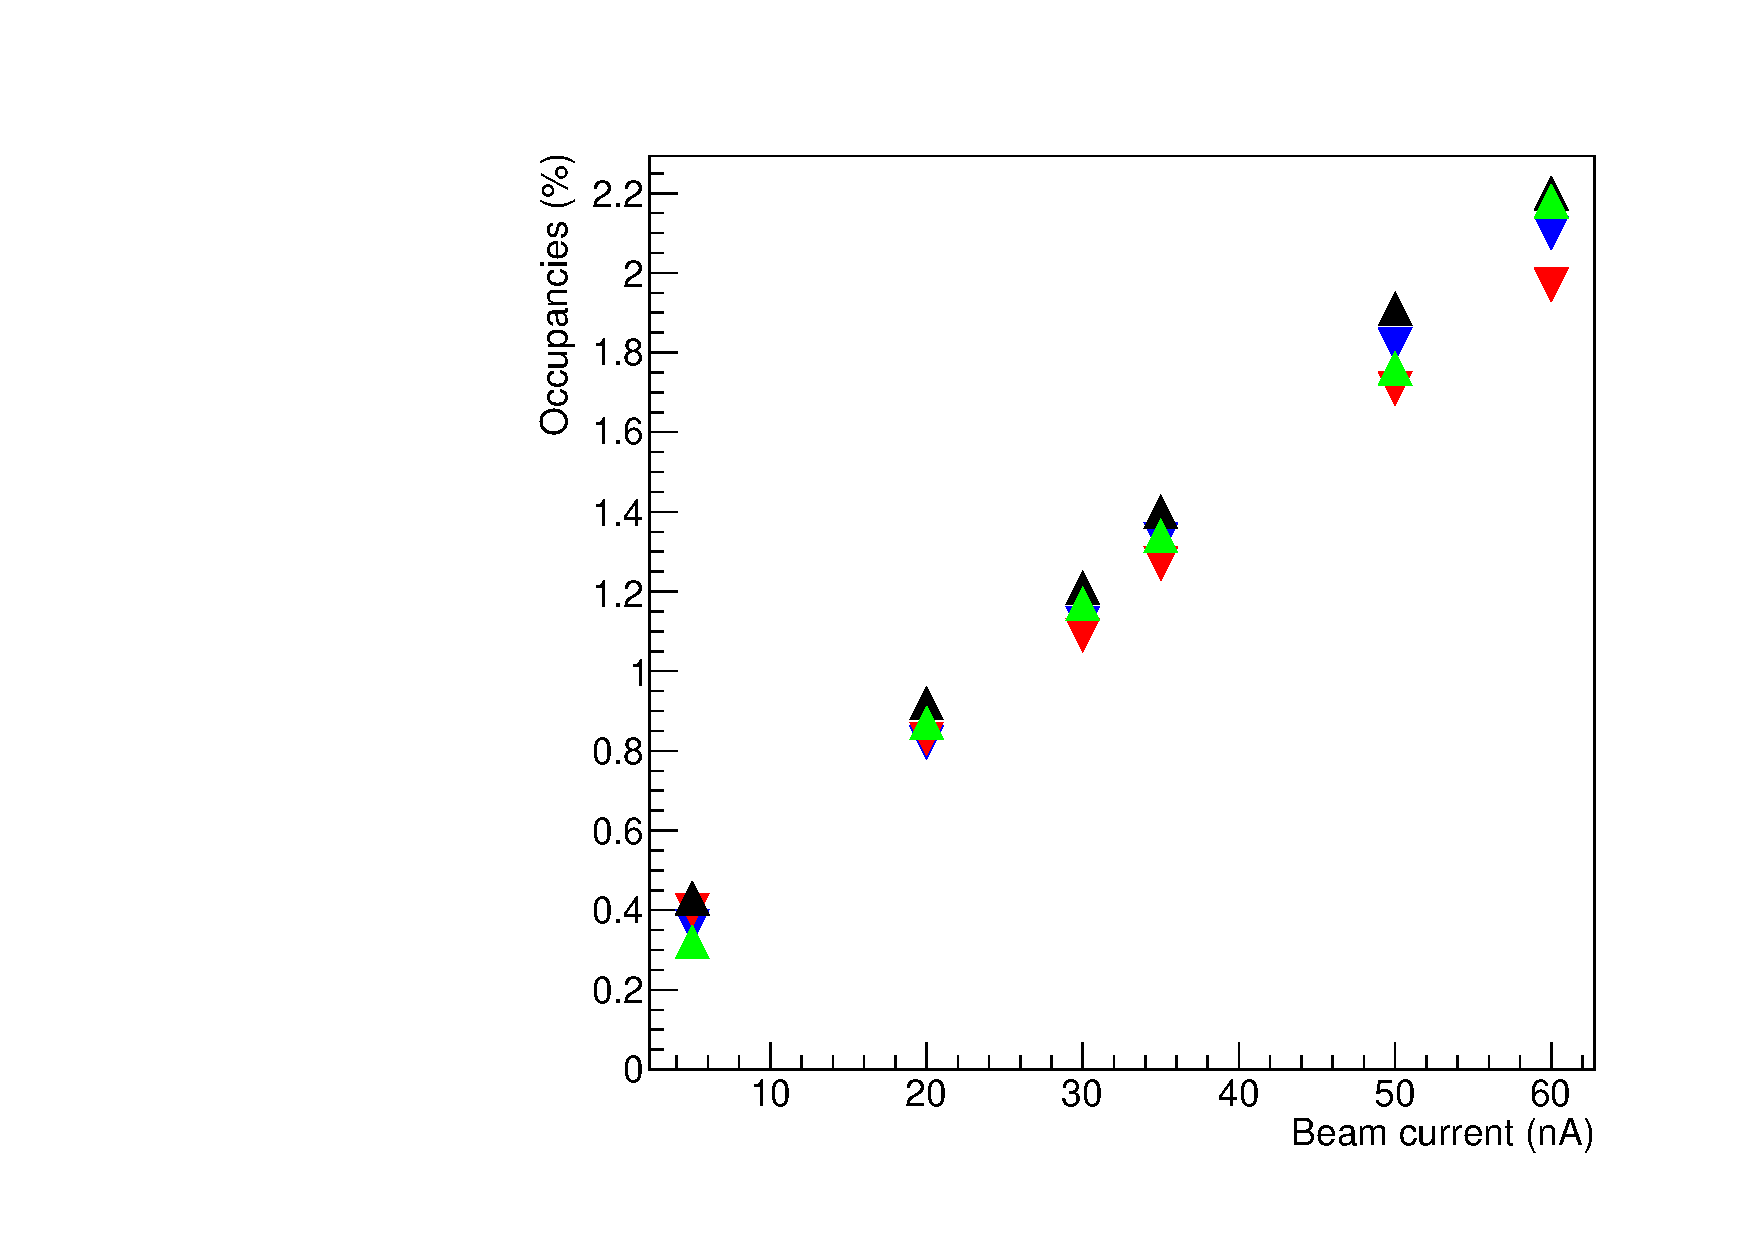
\includegraphics[width=.49\columnwidth,keepaspectratio]{images/OccupanciesVSbeamCurrent_BMT_only4Layers.pdf}
 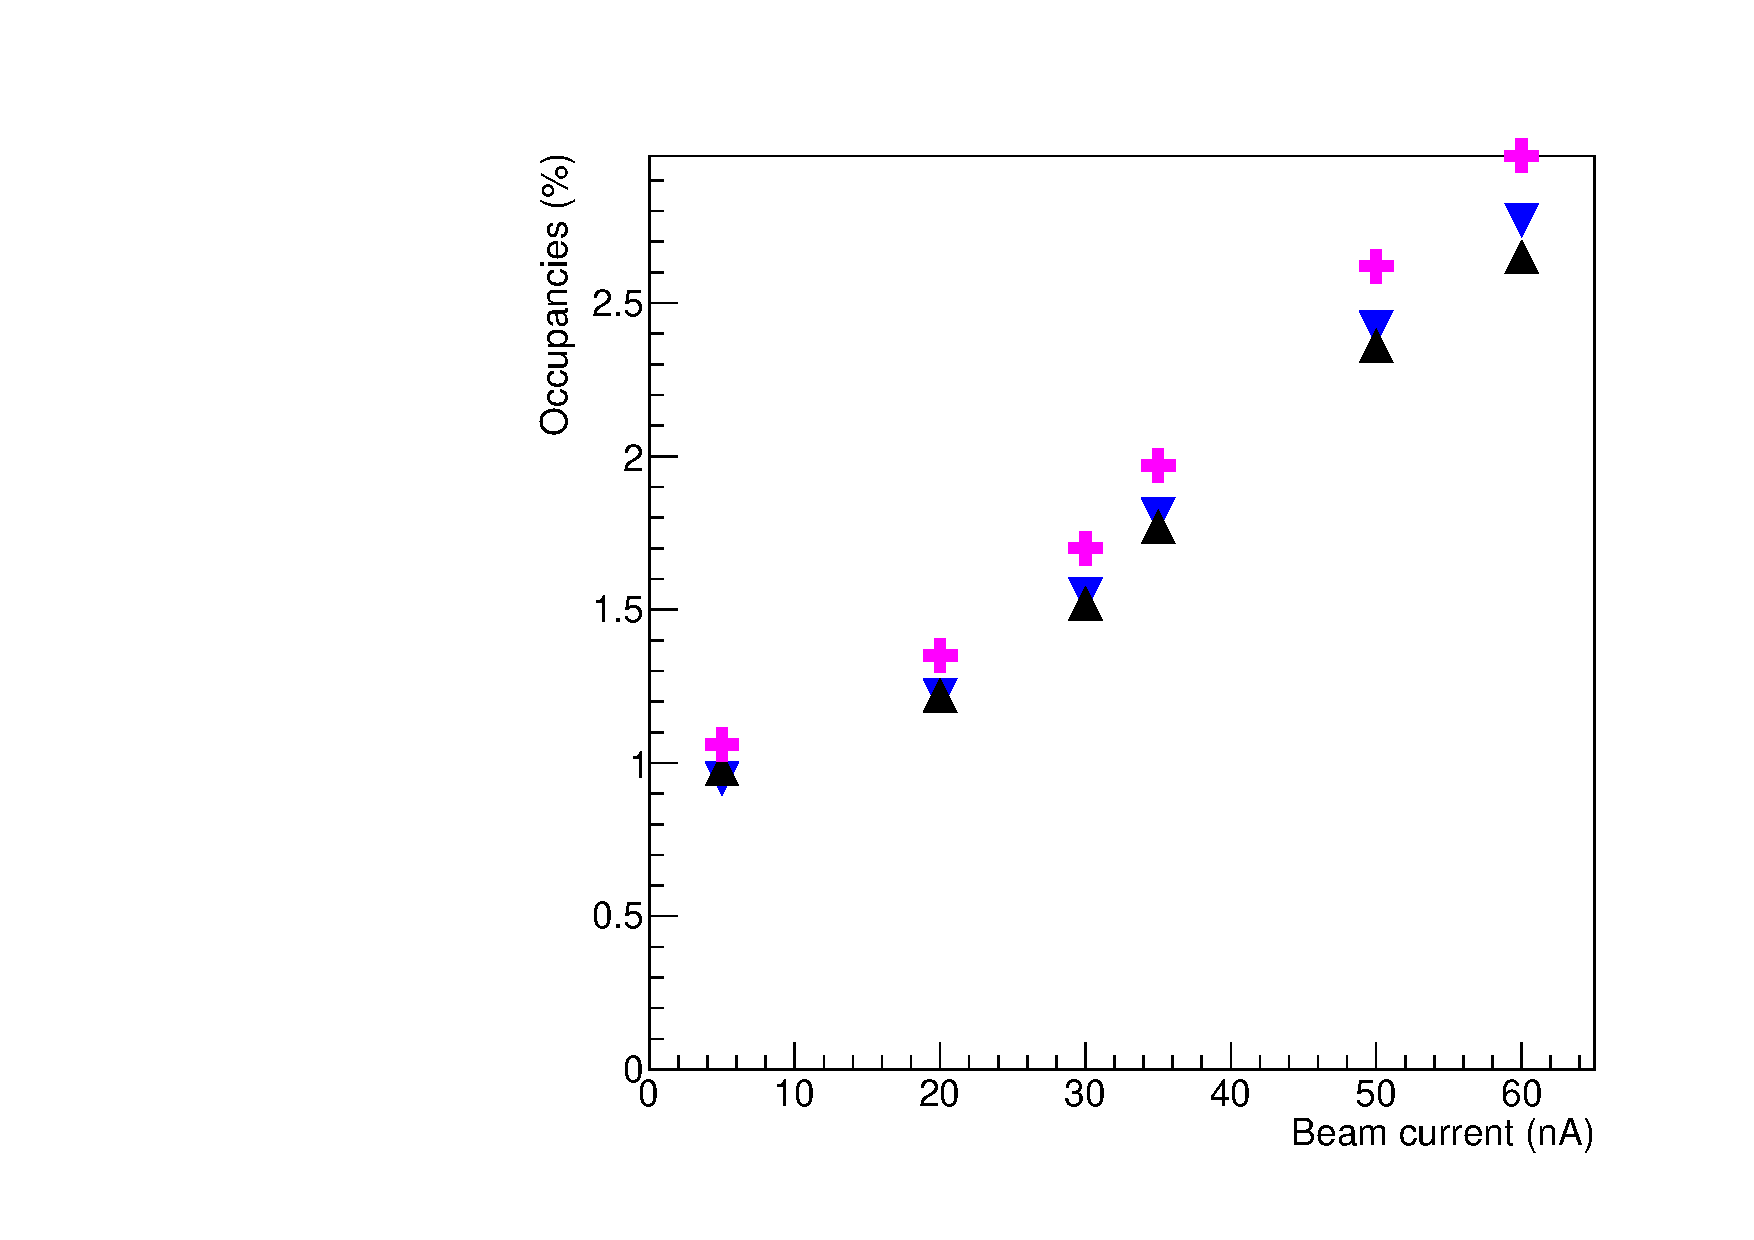
\includegraphics[width=.49\columnwidth,keepaspectratio]{images/OccupanciesVSbeamCurrent_FMT_only3Layers.pdf}
 \caption{Hit occupancy as a function of the beam current for 4 BMT layers (left) and 3 FMT disks (right).}
 \label{fig:mm-fig16}
\end{figure}

During the first year of operations with beam, CLAS12 took data at several electron beam energies (2.2, 6,4, 7.5, and 10.6~GeV)
with a liquid-hydrogen target. An example of a rare event at 10.6~GeV with five tracks reconstructed in the CVT is 
shown in Figure~\ref{fig:cd-tracks}. At 2.2~GeV, the large elastic cross section and the trigger configuration allowed 
for the visualization of the recoil protons in the raw occupancies of the BMT-C tiles as seen in 
Fig.~\ref{fig:mm-occupancy_22_10}. 

\begin{figure}[htb]
 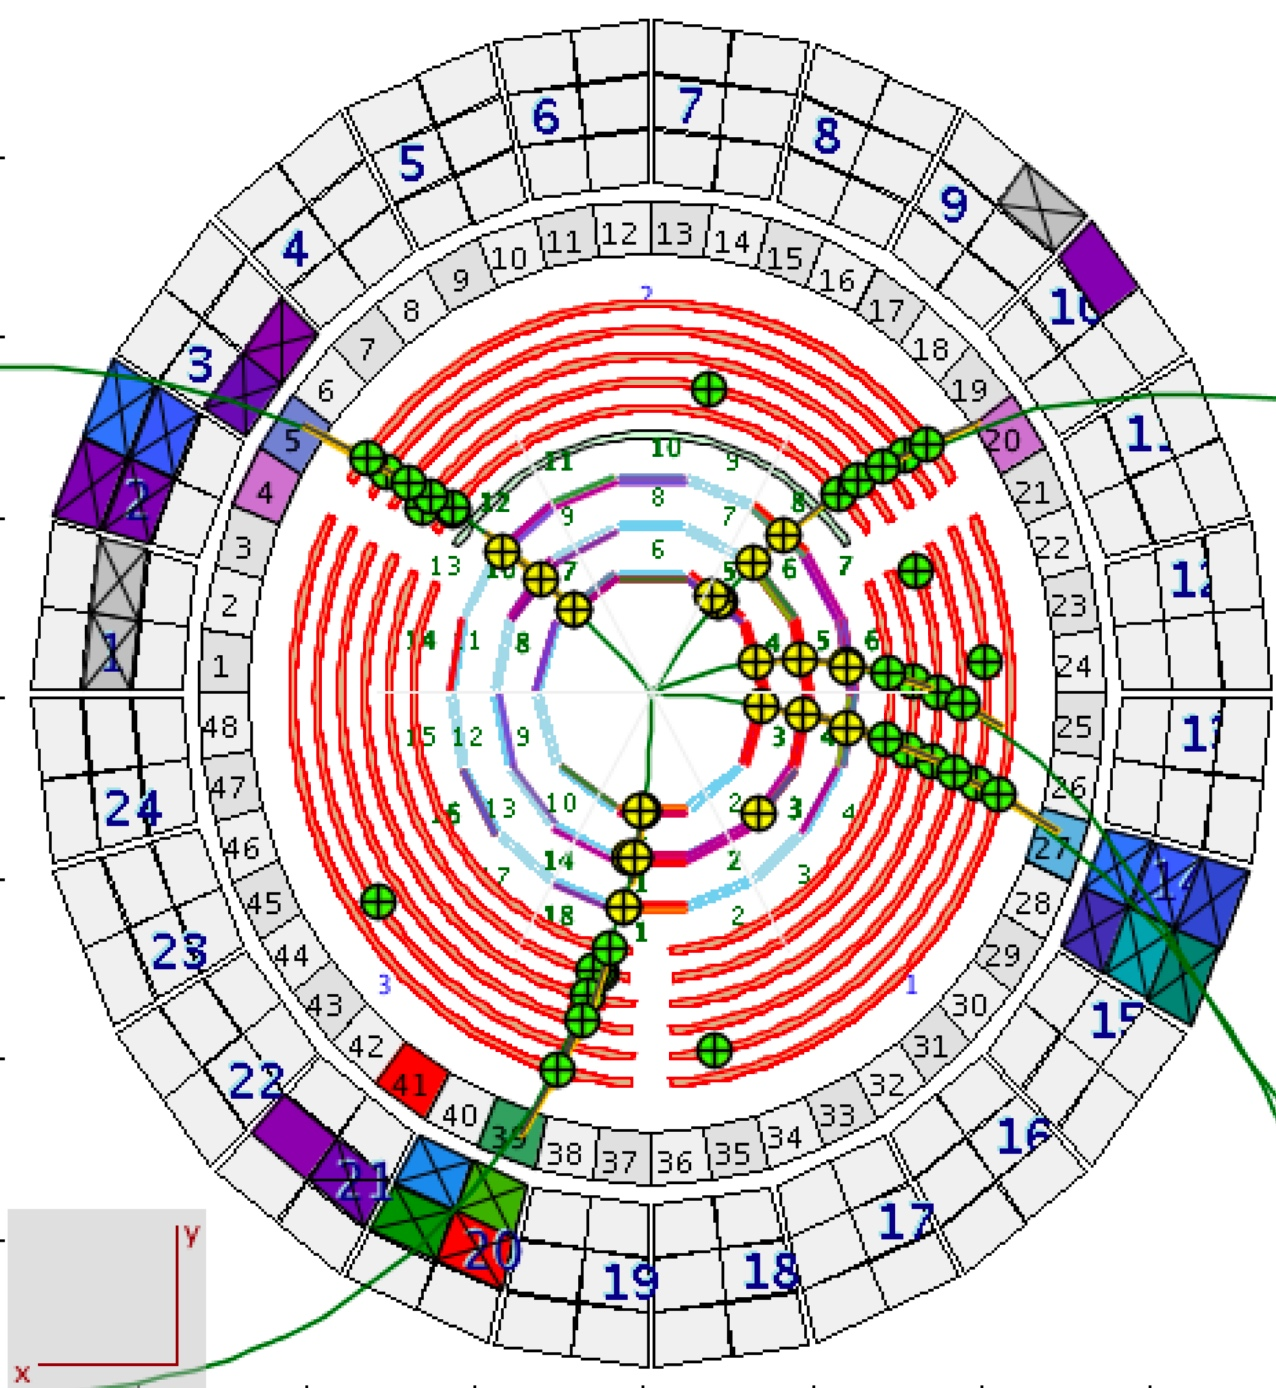
\includegraphics[width=.9\columnwidth]{images/cd-tracks}
 \caption{Event display of a rare five-track event in the CVT.}
 \label{fig:cd-tracks}
\end{figure}


\begin{figure}[htb]
 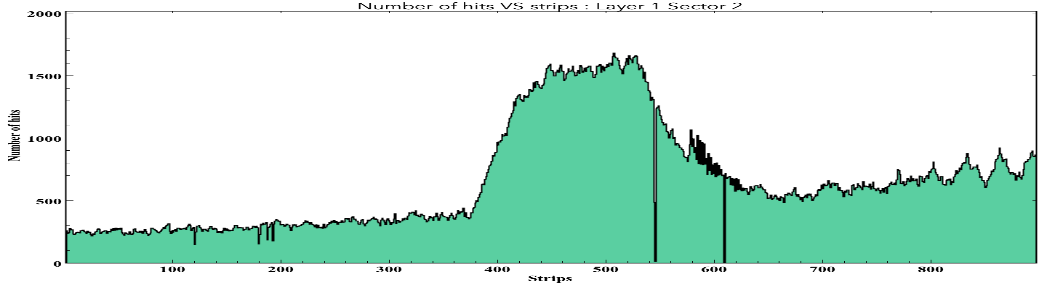
\includegraphics[width=1.0\columnwidth]{images/occupancy2GeV}
 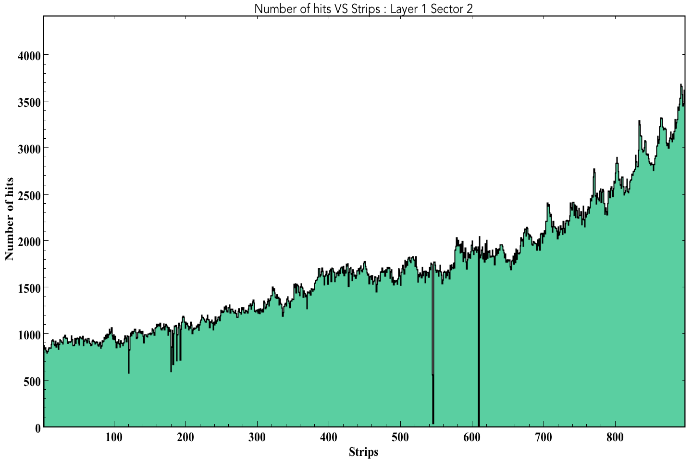
\includegraphics[width=1.0\columnwidth]{images/occupancy10GeV}
 \caption{Hit occupancy for C-tiles at 2.2~GeV (top) and 10.6~GeV (bottom) in events triggered by an electron in the forward
   CLAS12 detectors. The elastic recoil protons are responsible for the large excess of events at 2.2~GeV between strip number
   400 and 700. At 10.6~GeV, the elastic cross section is too small and no clear proton excess is visible.}
 \label{fig:mm-occupancy_22_10}
\end{figure}

The largest data set has been collected at an electron beam energy of 10.6~GeV and at 50~nA intensity.
Figure~\ref{fig:mm-beam_cls} shows the distributions of the number of clusters on all the six BMT layers and their cluster size
distribution. Although most of the events present a very low number of clusters with clusters of small size, the long tails are mainly
due to knock-off electron loopers and beam induced soft photons.

\begin{figure}[htb]
 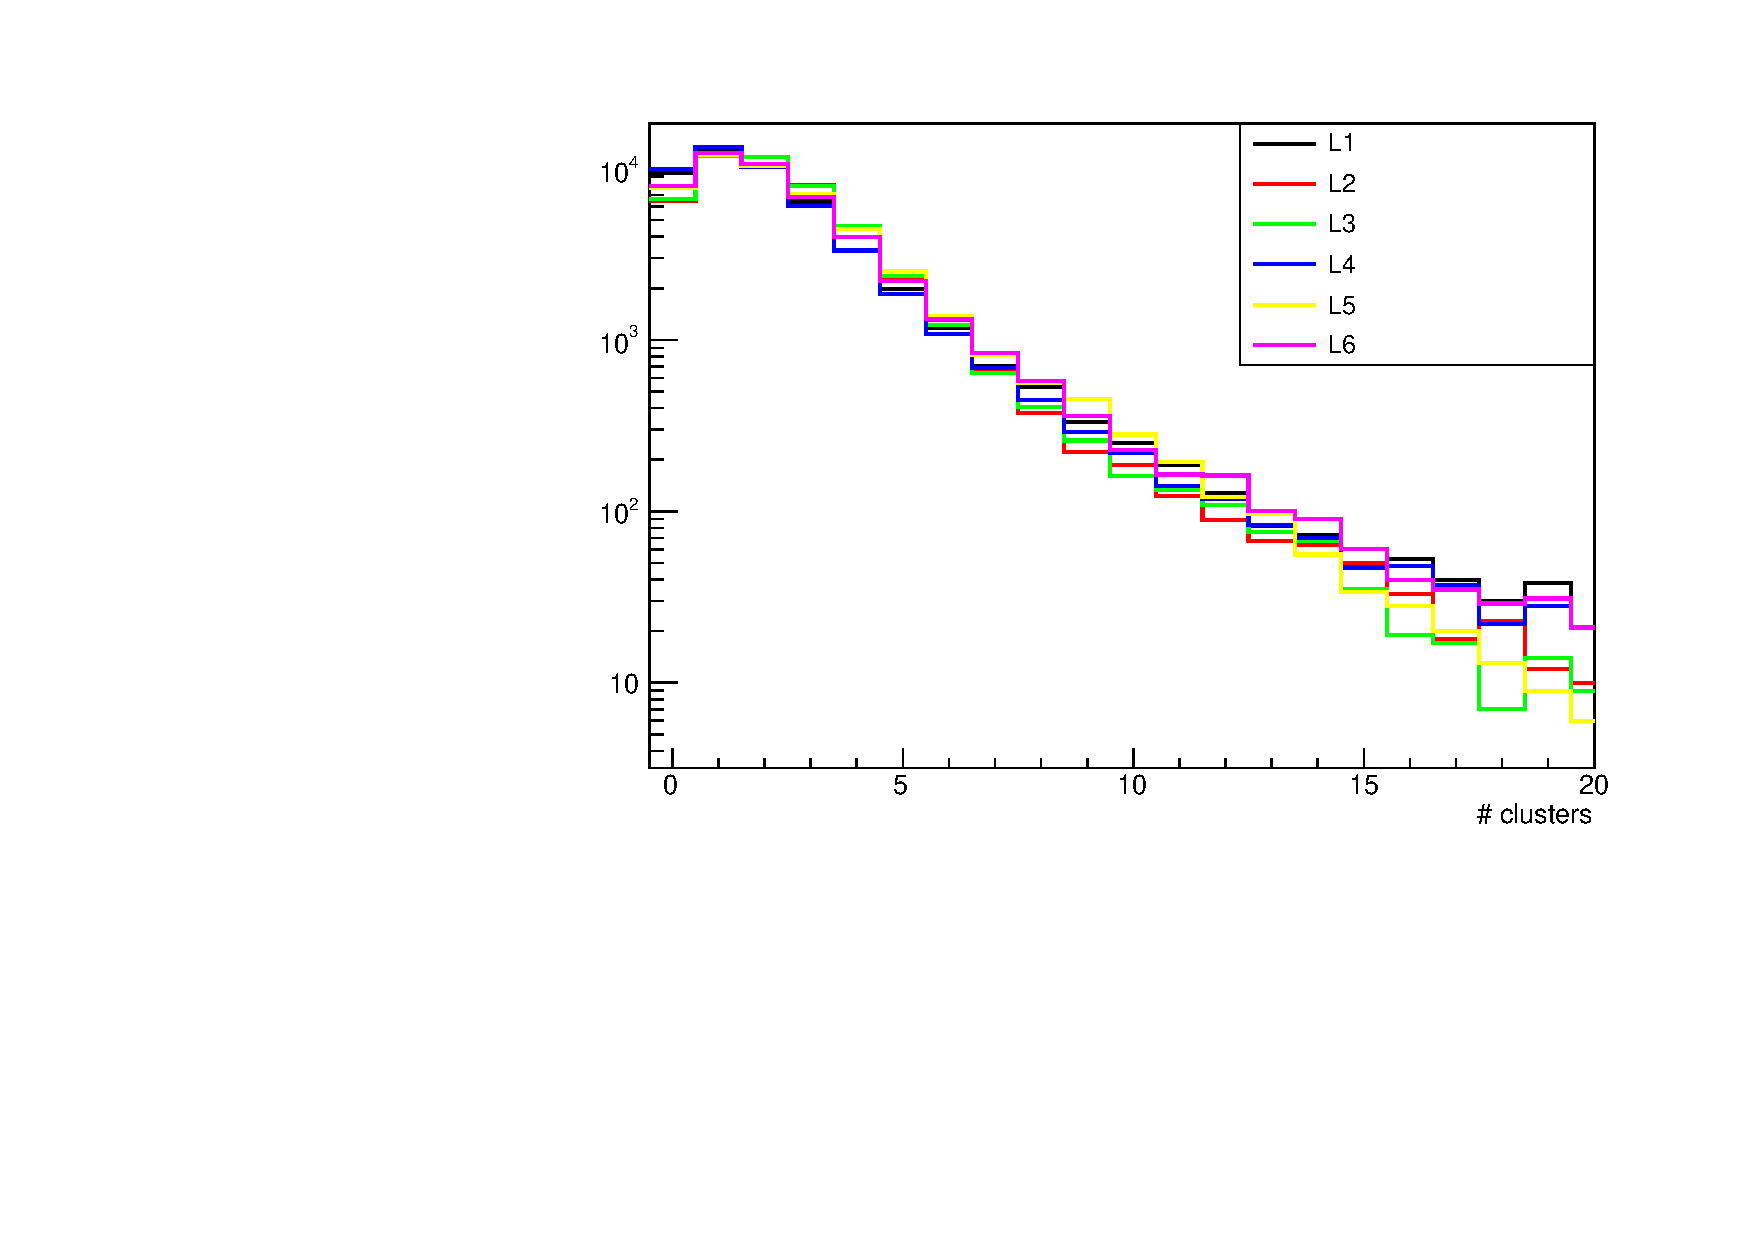
\includegraphics[width=.49\columnwidth,keepaspectratio]{images/beam_num_cls.pdf}
 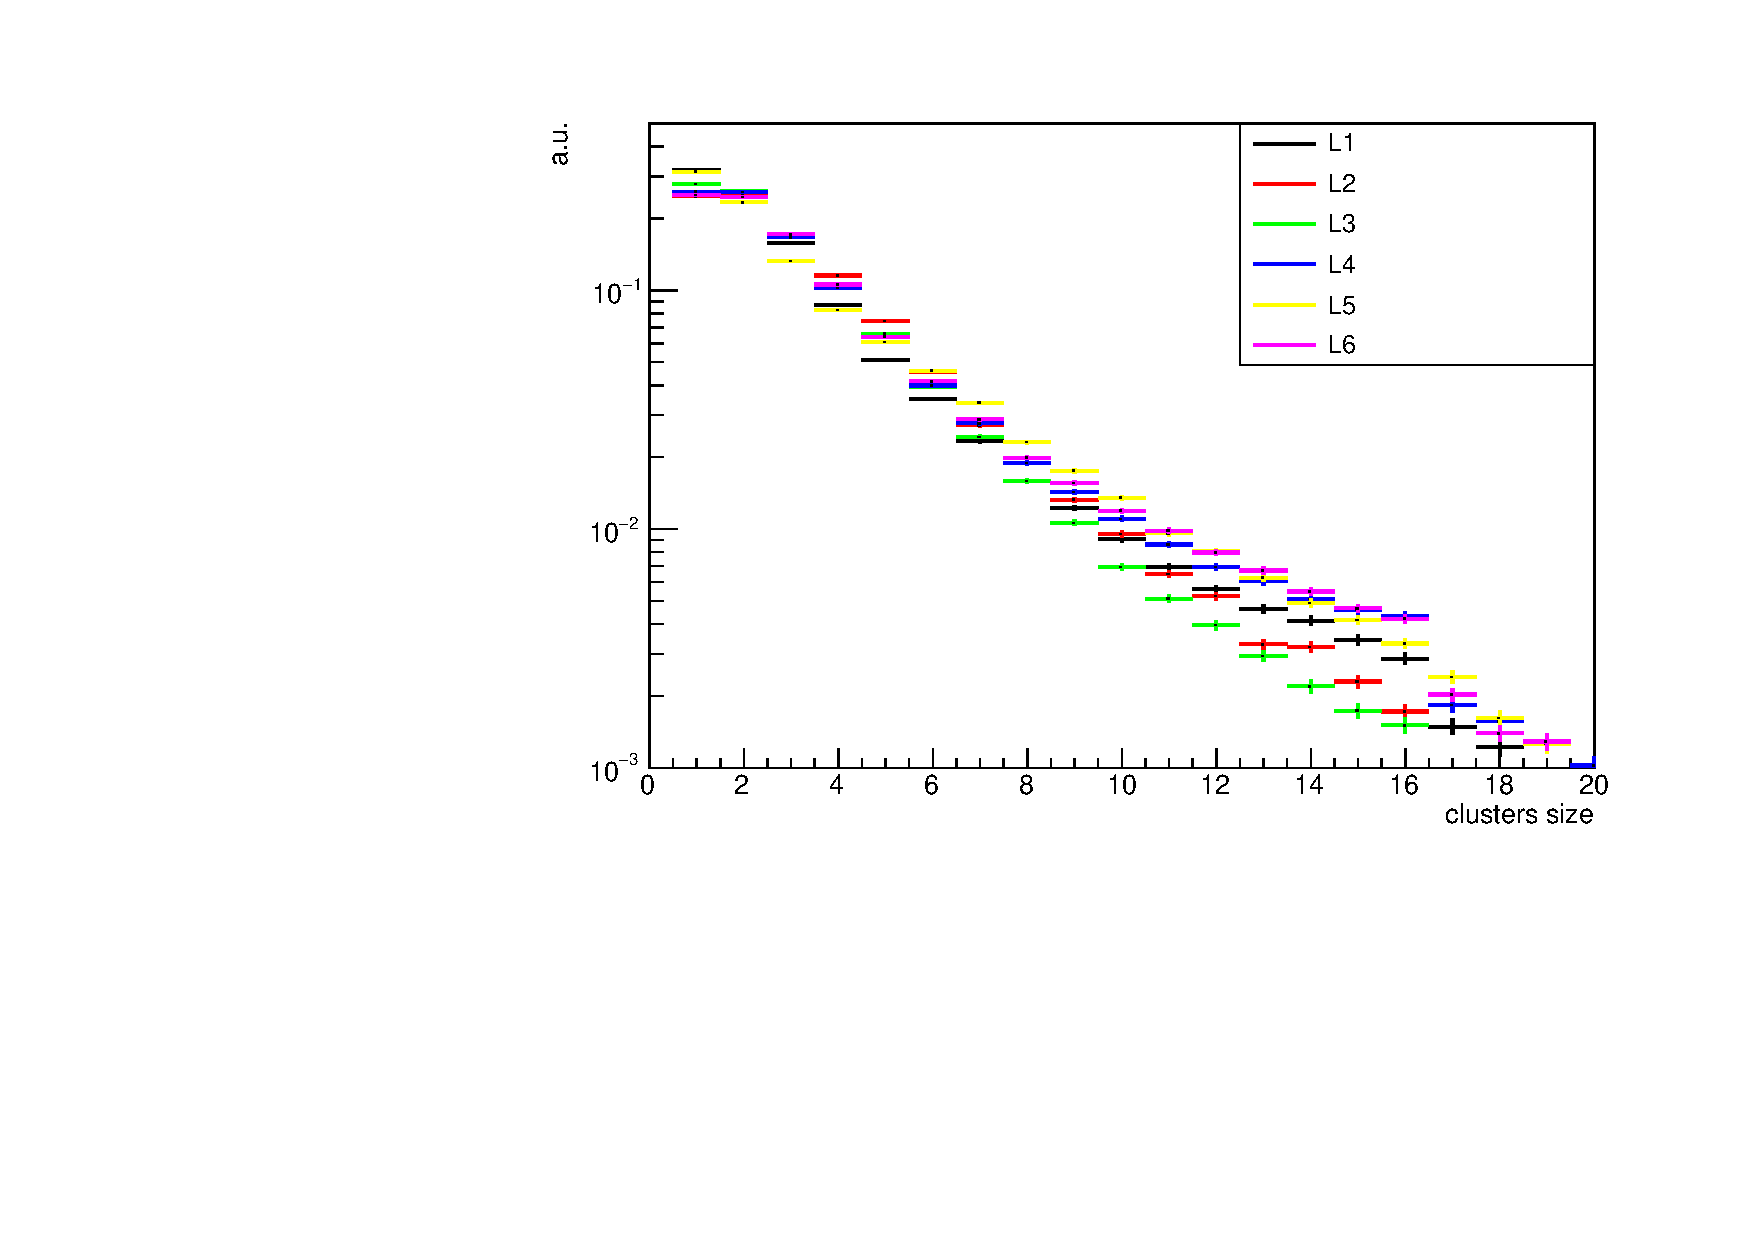
\includegraphics[width=.49\columnwidth,keepaspectratio]{images/beam_cls_size.pdf}
 \caption{(left) Number of clusters per event and (right) cluster size distribution in the BMT layers. The beam current was 50~nA.}
 \label{fig:mm-beam_cls}
\end{figure}

Each MVT hit has an associated timestamp that can be used to compute the time difference of the signal with respect to the
trigger. Consequently, a minimum time T$_{min}$ can be associated with each cluster as the minimum time of the hits in the cluster.
Figure~\ref{fig:mm-beam_cls_time} clearly shows that the clusters that have been associated with a reconstructed track have
a similar T$_{min}$ distributions over the six BMT layers, i.e. the clusters associated with a triggered physics event are strongly
correlated in time. However, the T$_{min}$ distributions of background clusters that are not associated with reconstructed tracks
show a peak toward lower values due to charged particles produced out of time with respect to the trigger signal.

\begin{figure}[htb]
 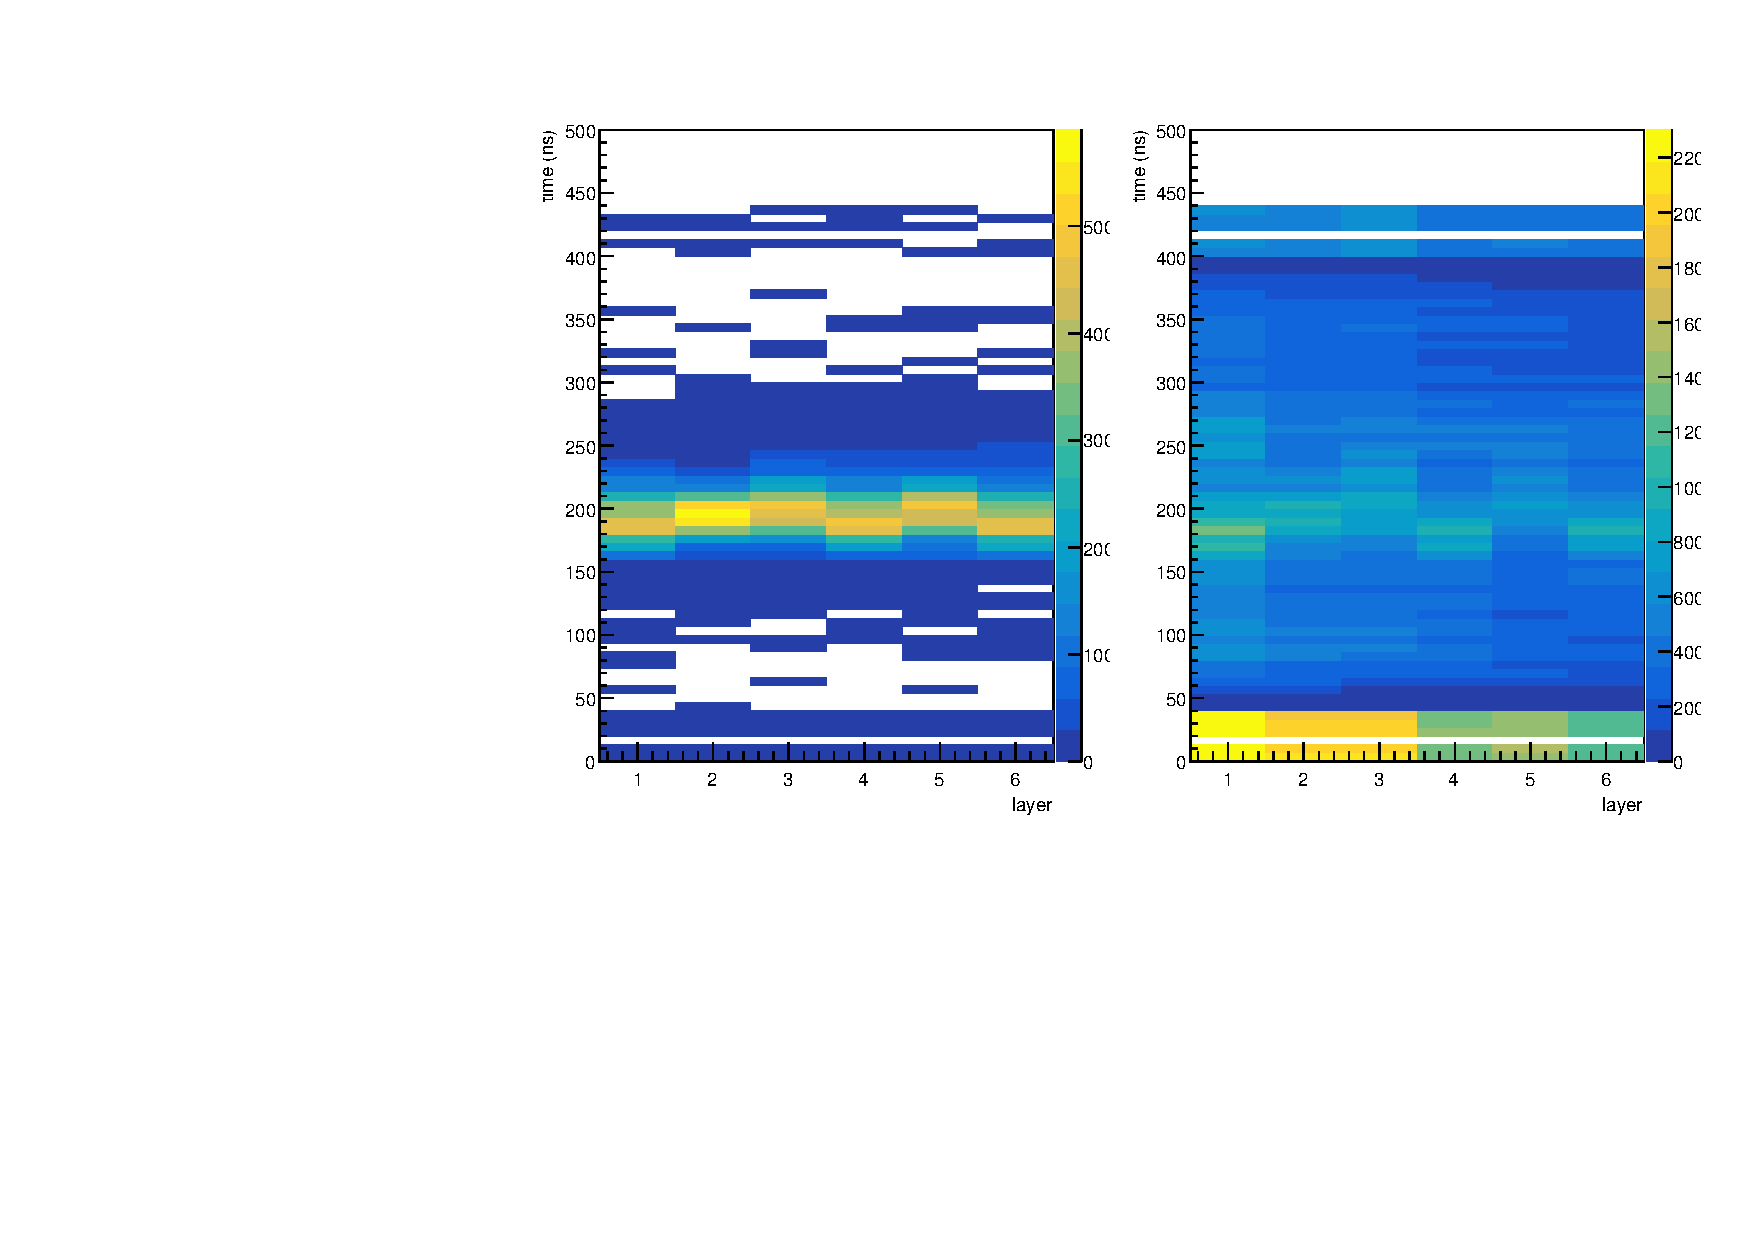
\includegraphics[width=\columnwidth,keepaspectratio]{images/align_cls_time.pdf}
 \caption{(left) Time distribution in the six BMT layers for clusters associated with a track; (right) Time distribution for clusters
   not associated with a reconstructed track.}
 \label{fig:mm-beam_cls_time}
\end{figure}

Special data taking periods with an empty target cell have been performed for calibration purposes, as well as low luminosity runs
with zero magnetic field for detector alignment studies. The stand-alone straight-track algorithm used for cosmic ray
reconstruction has been adapted and extended to use SVT hits. Using preliminary alignment corrections for both the SVT and
BMT, a zero-field empty-target run was reconstructed in SVT-stand-alone mode and CVT (i.e. SVT$+$BMT) mode. The 
preliminary resulsts shown in Fig.~\ref{fig:mm-zvertex}, the aluminum target walls are clearly visible in both 
reconstruction modes. It is possible to note that there is a significant improvement from $\sim$4.5~mm to 2.5~mm of the 
vertex position along the beam axis when the BMT information is used in the track reconstruction. Indeed the BMT-C tiles 
largely improve the polar angle of the particle with respect to the SVT-stand-alone mode. Concerning the azimuthal 
angle, the resolution of the BMT-Z tiles is not as good from the SVT modules and they are further away from the beam 
axis. Therefore the improvement of the resolution on the azimuthal angle of the track and related quantities like the 
vertex transverse coordinates is limited. On the other hand, the BMT-Z tiles provide an essential redundancy for tracks that 
cross a limited number of SVT layers.

\begin{figure*}[htb]
 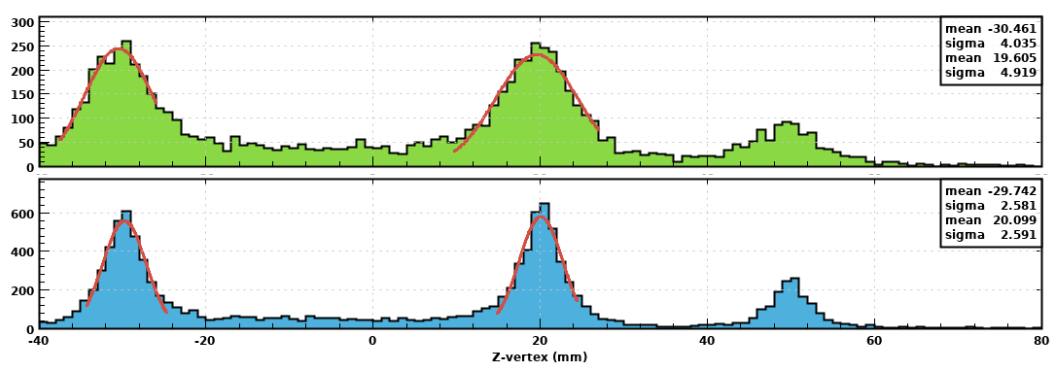
\includegraphics[width=2.0\columnwidth,keepaspectratio]{images/NIM_SVTvsCVT.png}
 \caption{Perliminary vertex position along the beam axis reconstructed with SVT-stand-alone reconstruction (top-green 
distribution) and    CVT reconstruction (bottom-blue distribution) for an empty-target and no solenoid field. The 
target walls are located at    -30 and 20~mm with gaseous hydrogen in-between. At 50~mm, the scattering chamber cap is 
clearly visible. The improvement in the resolution from SVT to CVT reconstruction is mainly due to the BMT-C tiles.}
 \label{fig:mm-zvertex}
\end{figure*}
